\section{Συνεχής τυχαίος περίπατος σε δύο διαστάσεις-Μέση Τετραγωνική Απόσταση}
Στην συνέχεια των πειραμάτων με σωματίδιο σε τυχαίο περίπατο θα προσομοιώσουμε ένα συνεχή χώρο και όχι σε ένα πλέγμα με ακέραιες τιμές. Ο τρόπος να προσεγγίζουμε συνεχής χώρους υπολογιστικά είναι να δεχτούμε μικρές υποδιαιρέσεις των παραμέτρων. Ένα δισδιάστατο χώρο μπορούμε να τον παραμετροποιήσουμε με χρήση πολικών συντεταγμένων. Ο τρόπος με τον οποίο θα ανανεώνεται η θέση του σωματιδίου στον συνεχή χώρο είναι με την τυχαία επιλογή γωνίας. Χωρίζουμε το επίπεδο σε 360 ίσες διαμερίσεις ενός κυκλικού δίσκου. Επομένως, για ένα πείραμα, θα έχουμε μία επανάληψη χιλίων βημάτων και θα επιλέγουμε τυχαία μία γωνία. Συνεπώς ο αλγόριθμος θα έχει τη μορφή:
\en
\begin{lstlisting}
//=============================================================//
set starting position 
For t=1000 steps:
    choose randomly(uniformly) an angle 
    update particle position based on that angle
//=============================================================//
\end{lstlisting}
\gr 
\todo{Εικόνα επεξηγηματική}
Για την τυχαία επιλογή της γωνίας εκμεταλλευόμαστε την εντολή { \en random.randint(0,359)} για την επιλογή σε μοίρες και μετατρέπουμε σε {\en rad} με χρήση του τύπου: 
\begin{equation}
\frac{angle}{180}=\frac{rad}{\pi}
\end{equation}
άρα:
\en
\begin{python}
angle = (random.randint(0,359)/180)*np.pi
\end{python}
\gr 
Η ανανέωση της θέσης γίνεται προβάλλοντας το ευθύγραμμο τμήμα μήκους {\en step}=1 στον άξονα $x$ πολλαπλασιάζοντας με το συνημίτονο της γωνίας, και στον άξονα $y$ πολλαπλασιάζοντας με το ημίτονο της γωνίας.

Συνεπώς για ένα πείραμα κώδικας έχει τη μορφή:
\en 
\begin{python}
position_x = 0
position_y = 0
for j in range(t):
    angle = (random.randint(0,359)/180)*np.pi
    position_x+=round(step*np.cos(angle),2)
    position_y+=round(step*np.sin(angle),2)
\end{python}
\gr όπου η συνάρτηση {\en round} στρογγυλοποιεί τους υπολογισμούς των  τριγωνομετρικών στο δεύτερο δεκαδικό.
Εφόσον θέλουμε να υπολογίσουμε ξανά την μέση τετραγωνική μετατόπιση, τρέχουμε τον κώδικα για {\en runs}=100000 πειράματα και προσθέτουμε την τετραγωνική απόσταση από την αρχή των αξόνων(την αρχική μας θέση) σύμφωνα με το πυθαγόρειο θεώρημα. Στο τέλος διαιρούμε το άθροισμα με τον αριθμό των πειραμάτων για να βρούμε τη μέση τιμή. Ο συνολικός κώδικας έχει ως εξής:
\en
\begin{python}
start_time = time.time()

sd_sum = 0
runs = 100000
t=1000
step = 1
for i in range(runs):
    position_x = 0
    position_y = 0
    for j in range(t):
        angle = (random.randint(0,359)/180)*np.pi
        position_x+=round(step*np.cos(angle),2)
        position_y+=round(step*np.sin(angle),2)
    sd_sum+=position_x**2+position_y**2
mean_sd = sd_sum/runs

print(f"The Mean Square Displacement is {mean_sd}.")
print(f"Execution Time: {(time.time() - start_time)} seconds.")
\end{python}
\gr με \en output:
\begin{python}
The Mean Square Displacement is 999.8212898829913.
Execution Time: 963.7810792922974 seconds.
\end{python}
\gr 
Τώρα θα υπολογίσουμε ξανά την μέση τετραγωνική μετατόπιση αλλά αυτή τη φορά θα πάρουμε τους μέσους όρους των 100000 πειραμάτων ανά 100 τυχαία βήματα. Δηλαδή θα βρούμε την μέση τετραγωνική μετατόπιση από 100000 πειράματα με 100 βήματα, την μέση τετραγωνική μετατόπιση από 100000 πειράματα με 200 βήματα κ.ο.κ. Η βασική δομή του κώδικα είναι όμοια με το προηγούμενο πείραμα σε συνεχές χώρο αλλά με κάποιες τροποποιήσεις.

 Αρχικοποιούμε μία λίστα 10 θέσεων ονόματι {\en averages} με την τιμή μηδέν σε κάθε στοιχείο της. Σε αυτή τη λίστα θα προσθέτουμε τις τιμές της τετραγωνικής μετατόπισης για τα 100,200,300....1000 βήματα και θα διαιρούμε με τον αριθμό των πειραμάτων προκειμένου να έχουμε τις μέσες τιμές ανά αριθμό βημάτων.
 
Το σχήμα του αλγορίθμου ενός πειράματος έχει ως εξής: 
\en
\begin{lstlisting}
//=============================================================//
set starting position 
create an empty list named values

For 1000 steps:
    choose randomly(uniformly) an angle 
    update particle position based on that angle
    if steps are 100,200......1000 
              then fill the list values
              with the square displacement
//=============================================================//
\end{lstlisting}
\gr 
Ο κώδικας που υλοποιεί το ένα πείραμα είναι:
\en
\begin{python}
position = [0,0]
values = []
for j in range(1,t+1):
    angle = (random.randint(0,359)/180)*np.pi
    position[0]+=round(np.cos(angle),2)
    position[1]+=round(np.sin(angle),2)
    if j%100==0:
        values.append(position[0]**2+position[1]**2)
\end{python}
\gr 
Λεπτομερέστερα, το {\en block} κώδικα:
\en
\begin{python}
if j%100==0:
    values.append(position[0]**2+position[1]**2)
\end{python}
\gr ελέγχει πότε ο αριθμός των βημάτων είναι πολλαπλάσιο του 100 (κοιτώντας να μηδενίζεται το υπόλοιπο της διαίρεσης με το 100) και γεμίζει την λίστα {\en values} με τις 10 τετραγωνικές μετατοπίσεις όπως φαίνεται και στον ψευδοκώδικα. Ο λόγος που επιλέχθηκε το {\en range(1,t+1)} και όχι το {\en range(0,t)} είναι καθαρά για την ευκρίνεια του κώδικα και τη χρήση του {\en mod100} αντί του {\en mod99}.

Έτσι για κάθε ένα πείραμα πρέπει να προσθέσουμε στην αρχικοποιημένη με μηδενικά λίστα {\en averages} τις τιμές της λίστας {\en values} διαιρεμένες με τον αριθμό των πειραμάτων προκειμένου να έχουμε στο τέλος τις μέσες τετραγωνικές μετατοπίσεις 100000 πειραμάτων ανά 100 βήματα του σωματιδίου.

Ο τελικός κώδικας θα είναι: \en
\begin{python}
start_time = time.time()

runs = 10000
t=1000
averages = [0]*10
for i in range(runs):
    position = [0,0]
    values = []
    for j in range(1,t+1):
        angle = (random.randint(0,359)/180)*np.pi
        position[0]+=round(np.cos(angle),2)
        position[1]+=round(np.sin(angle),2)
        if j%100==0:
            values.append(position[0]**2+position[1]**2)
    for j in range(10):
        averages[j]+=values[j]/runs

print(f"The averages are {averages}.")
print(f"Execution Time: {(time.time() - start_time)} seconds.")
\end{python}
\gr 
με έξοδο:
\en
\begin{python}
The averages are [99.67193910999949, 
                  201.10285323000062, 
                  298.58902693000033, 
                  399.82761215000033, 
                  494.9311487600011, 
                  597.2043227299978, 
                  693.3227494999987, 
                  791.3730152799965, 
                  901.8665181699997, 
                  1003.6801849000012].
Execution Time: 94.43011784553528 seconds.
\end{python}
\gr 
Χρησιμοποιούμε την μέθοδο ελαχίστων τετραγώνων μέσω του πακέτου {\en \texttt{sklearn.linear\_model}} και του αντικειμένου {\en LinearRegression()}. Αρχικά κατασκευάζουμε τα {\en np.array} αντικείμενα έτσι ώστε να μπορούν να εισαχθούν στις εντολές που θα χρησιμοποιήσουμε. Ως τετμημένες θα χρησιμοποιήσουμε τους αριθμούς των βημάτων που πραγματοποιήθηκαν στην μεταβλητή {\en t}. Η εντολή {\en  np.arange(100,1001,100).reshape(-1,1)} ουσιαστικά κατασκευάζει ένα στηλοδιάνυσμα με τα πολλαπλάσια του 100 έως και το 1000.  Ως τεταγμένες φυσικά τις μέσες τετραγωνικές μετατοπίσεις ανά 100 βήματα. Ο κώδικας:
\en
\begin{python}
t = np.arange(100,1001,100).reshape(-1,1)
av = np.array(averages)
\end{python}
\gr 
Εν συνεχεία, κατασκευάζουμε το μοντέλο γραμμικής παλινδρόμησης μέσω των μεθόδων που αναφέραμε, και στη συνέχεια εκτελούμε το {\en fitting}, δηλαδή το την εύρεση της ευθείας ελαχίστων τετραγώνων. Στη μεταβλητή {\en m} τοποθετούμε την κλίση της ευθείας και στην μεταβλητή {\en c} την σταθερά, έτσι ώστε η ευθείας μας να γράφετε ως $y = \mu t+c$. Ο κώδικας:
\en
\begin{python}
reg = LinearRegression()
model = reg.fit(t,av)
c = model.intercept_
m = model.coef_[0]
print(f"y = {m}x+{c}")
\end{python}
\gr 
με έξοδο
\en
\begin{python}
y = 0.999278690573332x+-1.4463427393329766
\end{python}
\gr 
Πλέον μένει να παραστήσουμε γραφικά την ευθεία και τα δεδομένα που χρησιμοποιήθηκαν προκειμένου να καταλήξουμε στα κατάλληλα συμπεράσματα.
Για να το κάνουμε αυτό θα χρησιμοποιήσουμε το πακέτο {\en matplotlib.pyplot} με το ακρωνύμιο {\en plt} όπως συνήθως χρησιμοποιείτε. Χρησιμοποιούμε την εξίσωση της ευθείας και την αναπαριστούμε γραφικά με γραμμή, ενώ τα αρχικά δεδομένα με τελείες. Ονομάζουμε τους άξονες και τα χρώματα σύμφωνα με το πρόβλημά μας. Ο τελικός κώδικας: 
\en
\begin{python}
y = m*t+c
plt.plot(t,y,'-',color ='green',label='Least Squares Regression Line')
plt.plot(t,av,'.',color = 'red',label='Data points',ms=10.0)
plt.legend()
plt.grid(color='0.25', linestyle='--', linewidth=0.2)
plt.ylabel('Square Displacement')
plt.xlabel('Number of Random Steps')
plt.title('Continuous Random Walk - Mean Square Displacement')
plt.show()
\end{python}
\gr και το {\en } γράφημα:
\begin{figure}[H]
\begin{center}
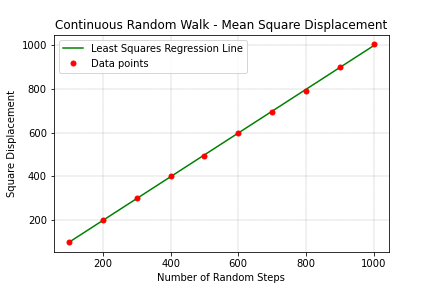
\includegraphics[scale=1]{figures/CRW_MSD.png}
\caption{Μέση τετραγωνική απόσταση αν 100 βηματισμούς του σωματιδίου για συνεχή χώρο δύο διατάσεων}
\label{figuridion3d}
\end{center}
\end{figure}
